
%%%%%%%%%%%%%%%%%%%%%%%%%%%%%%%%%%%%%%%%%
% Focus Beamer Presentation
% LaTeX Template
% Version 1.0 (8/8/18)
%
% This template has been downloaded from:
% http://www.LaTeXTemplates.com
%
% Original author:
% Pasquale Africa (https://github.com/elauksap/focus-beamertheme) with modifications by 
% Vel (vel@LaTeXTemplates.com)
%
% Template license:
% GNU GPL v3.0 License
%
% Important note:
% The bibliography/references need to be compiled with bibtex.
%
%%%%%%%%%%%%%%%%%%%%%%%%%%%%%%%%%%%%%%%%%

%----------------------------------------------------------------------------------------
%	PACKAGES AND OTHER DOCUMENT CONFIGURATIONS
%----------------------------------------------------------------------------------------

\documentclass{beamer}
\usepackage{enumitem}
\beamertemplatenavigationsymbolsempty % suppress navigation bar

\usetheme{default} % Use the Focus theme supplied with the template
% Add option [numbering=none] to disable the footer progress bar
% Add option [numbering=fullbar] to show the footer progress bar as always full with a slide count

% Uncomment to enable the ice-blue theme
%\definecolor{main}{RGB}{92, 138, 168}
%\definecolor{background}{RGB}{240, 247, 255}

%------------------------------------------------

\usepackage{booktabs} % Required for better table rules

\begin{document}

\begin{frame}{Questions}
Firms that emit toxins into the air without paying pollution taxes or purchases licenses to pollute tend to 
\begin{enumerate}[label=\alph*)]
\item Underproduce because the private cost of production exceeds the social cost
\item Overproduce because the social cost of production exceeds the private cost
\item Produce the same quantity as nonpolluting firms
\item Produce the socially optimal amount
\item "Internalize the externality" in the product's price
\end{enumerate}
\end{frame}

\begin{frame}{Questions}
In the economic analysis of negative externalities (e.g., toxins in the atmosphere)
\begin{enumerate}[label=\alph*)]
\item The optimal amount of the negative externality is \textbf{zero}
\item One considers the costs of reducing the toxins, not the benefits; environmentalists considier the benefits and not the costs
\item The private costs of an economic activity are \textbf{greater} than the social costs
\item The optimal amount of the externality is determined where MSC is equal to MSB
\item A proper application of corrective taxes will \textbf{reduce} the price that consumers pay for the externality-generating good.
\end{enumerate}
\end{frame}

\begin{frame}{The Coase Theorem}
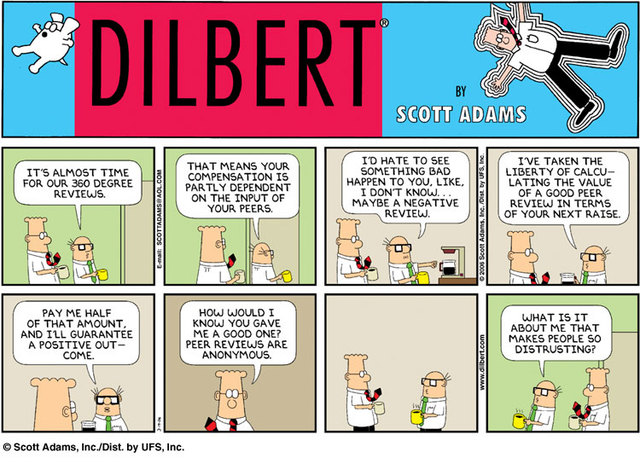
\includegraphics[width = \textwidth]{images/coasedilbert.jpg}
\end{frame}

\begin{frame}{The Coase Theorem}

\includegraphics[width = \textwidth]{images/coaseriver.png}
\end{frame}

\begin{frame}{The Coase Theorem}
\centering

\includegraphics[width = \textwidth]{images/coaseemissions.png}
\end{frame}




\end{document}
